\documentclass{ximera}

\outcomes{What is area?}
\outcomes{How do we find area under a curve?}
\outcomes{What do all the components of the formula mean?}
\outcomes{What is sigma notation and what does it mean?}
\outcomes{What are grid points and how do they help us compute area?} 
\outcomes{How do we know which rectangle we are on?}
\outcomes{What are the lengths and widths of the rectangles?}
\outcomes{Add up a large number of terms quickly using sigma notation.}
\outcomes{Approximate area under a curve.}
\outcomes{Approximate displacement from velocity.}
\outcomes{Compute left, right, and midpoint Riemann Sums.}

\title{Approximating area under curves}

\begin{document}

\begin{abstract}
	We can approximate the area under a curve by the sum of the areas of a bunch of rectangles.	
\end{abstract}

\maketitle

We have been studying differential calculus, the basic question of
which is ``What is the slope of the tangent line to a function at a
point?.''  

We now turn to \textbf{integral} calculus, the basic
question of which is "What is the (signed) area bounded by the graph
of a function?"

Our basic approach will be to approximate the area under a curve with
a sum of areas of rectangles.

\begin{question}
  Let $f(x) = x^2+1$.  Divide the interval $[0,1]$ into $3$
  subintervals of equal width.  Base a rectangle on each subinterval,
  whose height is given by the function value at the left endpoint.
  Then the sum of the areas of these rectangles is a (crude)
  approximation of the area under $f$ on the interval $[0,1]$.

\begin{image}
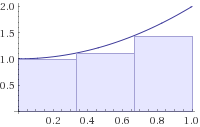
\includegraphics{riemann1.png}
\end{image}
	
  The sum of the areas of these rectangles is \answer{
    (1+(1+1/9)+(1+4/9))/3}
\end{question}

To write these kind of sums in a more compact notation, we introduce
sigma notation:

\begin{definition}
  Let $C(k)$ be a function which accepts integer inputs $k$.  Then if
  $a < b$, $\displaystyle\sum_{k=a}^{k=b} C(k)$ is defined to be the sum
  $C(a)+C(a+1)+C(a+2)+\dots +C(b-1)+C(b)$.
\end{definition}

\begin{example}
  $\displaystyle\sum_{k=2}^{k=5} k^2 = 2^2+3^2+4^2+5^2$
\end{example}

\begin{question}
	$\displaystyle\sum_{k=1}^{k=3} k = $\answer{6}
\end{question}

\begin{question}
  If we want to write the sum $(1+2(0))+(1+2(1))+(1+2(2))+(1+2(3))$ in
  sigma notation, in the form $\displaystyle\sum_{k=0}^{k=3} C(k)$, then
  $C(k)=$\answer{1+2k}
\end{question}

\begin{question}
  \begin{hint}
    All of the rectangles have width $\frac{1}{10}$.
  \end{hint}
  \begin{hint}
    The height of the third rectangle is $1+(\frac{2}{10})^2$.  Note that this corresponds to $k=2$, since we are counting $k=0,1,2,...$.  So the area of the rectangle corresponding to $k=2$ is $(1+(\frac{2}{10})^2) \cdot \frac{1}{10}$.
  \end{hint}
  Let $f(x) = x^2+1$.  Divide the interval $[0,1]$ into $10$ subintervals of equal width.  Base a rectangle on each subinterval, whose height is given by the function value at the left endpoint.  Then the sum of the areas of these rectangles is a (crude) approximation of the area under $f$ on the interval $[0,1]$.
	
\begin{image}
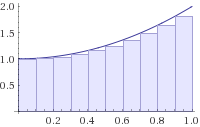
\includegraphics{riemann2.png}
\end{image}
	
  If we write the sum of the areas of these rectangles in sigma notation, in the form $\displaystyle \sum_{k=0}^{k=9} C(k)$, then $C(k) = $\answer{(1+k^2/100)/10}
\end{question}


\begin{question}
Write down at least \textbf{five} questions for this lecture. After
you have your questions, label them as ``Level 1,'' ``Level 2,'' or ``Level 3'' where:
\begin{description}
\item[Level 1] Means you know the answer, or know exactly how to do this problem.
\item[Level 2] Means you think you know how to do the problem, or will soon learn how to do the problem.
\item[Level 3] Means you have no idea how to do the problem. 
\end{description}
  \begin{freeResponse}
  \end{freeResponse}
\end{question}

\end{document}
